%!TeX root=../emmatop.tex
\chapter[Chapter \thechapter]{}
\lettrine[lraise=0.3]{M}{r} Elton must now be left to himself. It was no longer in Emma's power to superintend his happiness or quicken his measures. The coming of her sister's family was so very near at hand, that first in anticipation, and then in reality, it became henceforth her prime object of interest; and during the ten days of their stay at Hartfield it was not to be expected—she did not herself expect—that any thing beyond occasional, fortuitous assistance could be afforded by her to the lovers. They might advance rapidly if they would, however; they must advance somehow or other whether they would or no. She hardly wished to have more leisure for them. There are people, who the more you do for them, the less they will do for themselves.

Mr and Mrs John Knightley, from having been longer than usual absent from Surry, were exciting of course rather more than the usual interest. Till this year, every long vacation since their marriage had been divided between Hartfield and Donwell Abbey; but all the holidays of this autumn had been given to sea-bathing for the children, and it was therefore many months since they had been seen in a regular way by their Surry connexions, or seen at all by Mr Woodhouse, who could not be induced to get so far as London, even for poor Isabella's sake; and who consequently was now most nervously and apprehensively happy in forestalling this too short visit.

He thought much of the evils of the journey for her, and not a little of the fatigues of his own horses and coachman who were to bring some of the party the last half of the way; but his alarms were needless; the sixteen miles being happily accomplished, and Mr and Mrs John Knightley, their five children, and a competent number of nursery-maids, all reaching Hartfield in safety. The bustle and joy of such an arrival, the many to be talked to, welcomed, encouraged, and variously dispersed and disposed of, produced a noise and confusion which his nerves could not have borne under any other cause, nor have endured much longer even for this; but the ways of Hartfield and the feelings of her father were so respected by Mrs John Knightley, that in spite of maternal solicitude for the immediate enjoyment of her little ones, and for their having instantly all the liberty and attendance, all the eating and drinking, and sleeping and playing, which they could possibly wish for, without the smallest delay, the children were never allowed to be long a disturbance to him, either in themselves or in any restless attendance on them.

Mrs John Knightley was a pretty, elegant little woman, of gentle, quiet manners, and a disposition remarkably amiable and affectionate; wrapt up in her family; a devoted wife, a doating mother, and so tenderly attached to her father and sister that, but for these higher ties, a warmer love might have seemed impossible. She could never see a fault in any of them. She was not a woman of strong understanding or any quickness; and with this resemblance of her father, she inherited also much of his constitution; was delicate in her own health, over-careful of that of her children, had many fears and many nerves, and was as fond of her own Mr Wingfield in town as her father could be of Mr Perry. They were alike too, in a general benevolence of temper, and a strong habit of regard for every old acquaintance.

Mr John Knightley was a tall, gentleman-like, and very clever man; rising in his profession, domestic, and respectable in his private character; but with reserved manners which prevented his being generally pleasing; and capable of being sometimes out of humour. He was not an ill-tempered man, not so often unreasonably cross as to deserve such a reproach; but his temper was not his great perfection; and, indeed, with such a worshipping wife, it was hardly possible that any natural defects in it should not be increased. The extreme sweetness of her temper must hurt his. He had all the clearness and quickness of mind which she wanted, and he could sometimes act an ungracious, or say a severe thing.

He was not a great favourite with his fair sister-in-law. Nothing wrong in him escaped her. She was quick in feeling the little injuries to Isabella, which Isabella never felt herself. Perhaps she might have passed over more had his manners been flattering to Isabella's sister, but they were only those of a calmly kind brother and friend, without praise and without blindness; but hardly any degree of personal compliment could have made her regardless of that greatest fault of all in her eyes which he sometimes fell into, the want of respectful forbearance towards her father. There he had not always the patience that could have been wished. Mr Woodhouse's peculiarities and fidgetiness were sometimes provoking him to a rational remonstrance or sharp retort equally ill-bestowed. It did not often happen; for Mr John Knightley had really a great regard for his father-in-law, and generally a strong sense of what was due to him; but it was too often for Emma's charity, especially as there was all the pain of apprehension frequently to be endured, though the offence came not. The beginning, however, of every visit displayed none but the properest feelings, and this being of necessity so short might be hoped to pass away in unsullied cordiality. They had not been long seated and composed when Mr Woodhouse, with a melancholy shake of the head and a sigh, called his daughter's attention to the sad change at Hartfield since she had been there last.

<Ah, my dear,> said he, <poor Miss Taylor—It is a grievous business.>

<Oh yes, sir,> cried she with ready sympathy, <how you must miss her! And dear Emma, too!—What a dreadful loss to you both!—I have been so grieved for you.—I could not imagine how you could possibly do without her.—It is a sad change indeed.—But I hope she is pretty well, sir.>

<Pretty well, my dear—I hope—pretty well.—I do not know but that the place agrees with her tolerably.>

Mr John Knightley here asked Emma quietly whether there were any doubts of the air of Randalls.

<Oh! no—none in the least. I never saw Mrs Weston better in my life—never looking so well. Papa is only speaking his own regret.>

<Very much to the honour of both,> was the handsome reply.

<And do you see her, sir, tolerably often?> asked Isabella in the plaintive tone which just suited her father.

Mr Woodhouse hesitated.—<Not near so often, my dear, as I could wish.>

<Oh! papa, we have missed seeing them but one entire day since they married. Either in the morning or evening of every day, excepting one, have we seen either Mr Weston or Mrs Weston, and generally both, either at Randalls or here—and as you may suppose, Isabella, most frequently here. They are very, very kind in their visits. Mr Weston is really as kind as herself. Papa, if you speak in that melancholy way, you will be giving Isabella a false idea of us all. Every body must be aware that Miss Taylor must be missed, but every body ought also to be assured that Mr and Mrs Weston do really prevent our missing her by any means to the extent we ourselves anticipated—which is the exact truth.>

<Just as it should be,> said Mr John Knightley, <and just as I hoped it was from your letters. Her wish of shewing you attention could not be doubted, and his being a disengaged and social man makes it all easy. I have been always telling you, my love, that I had no idea of the change being so very material to Hartfield as you apprehended; and now you have Emma's account, I hope you will be satisfied.>

<Why, to be sure,> said Mr Woodhouse—<yes, certainly—I cannot deny that Mrs Weston, poor Mrs Weston, does come and see us pretty often—but then—she is always obliged to go away again.>

<It would be very hard upon Mr Weston if she did not, papa.—You quite forget poor Mr Weston.>

<I think, indeed,> said John Knightley pleasantly, <that Mr Weston has some little claim. You and I, Emma, will venture to take the part of the poor husband. I, being a husband, and you not being a wife, the claims of the man may very likely strike us with equal force. As for Isabella, she has been married long enough to see the convenience of putting all the Mr Westons aside as much as she can.>

\begin{figure}[tbph]
\centering
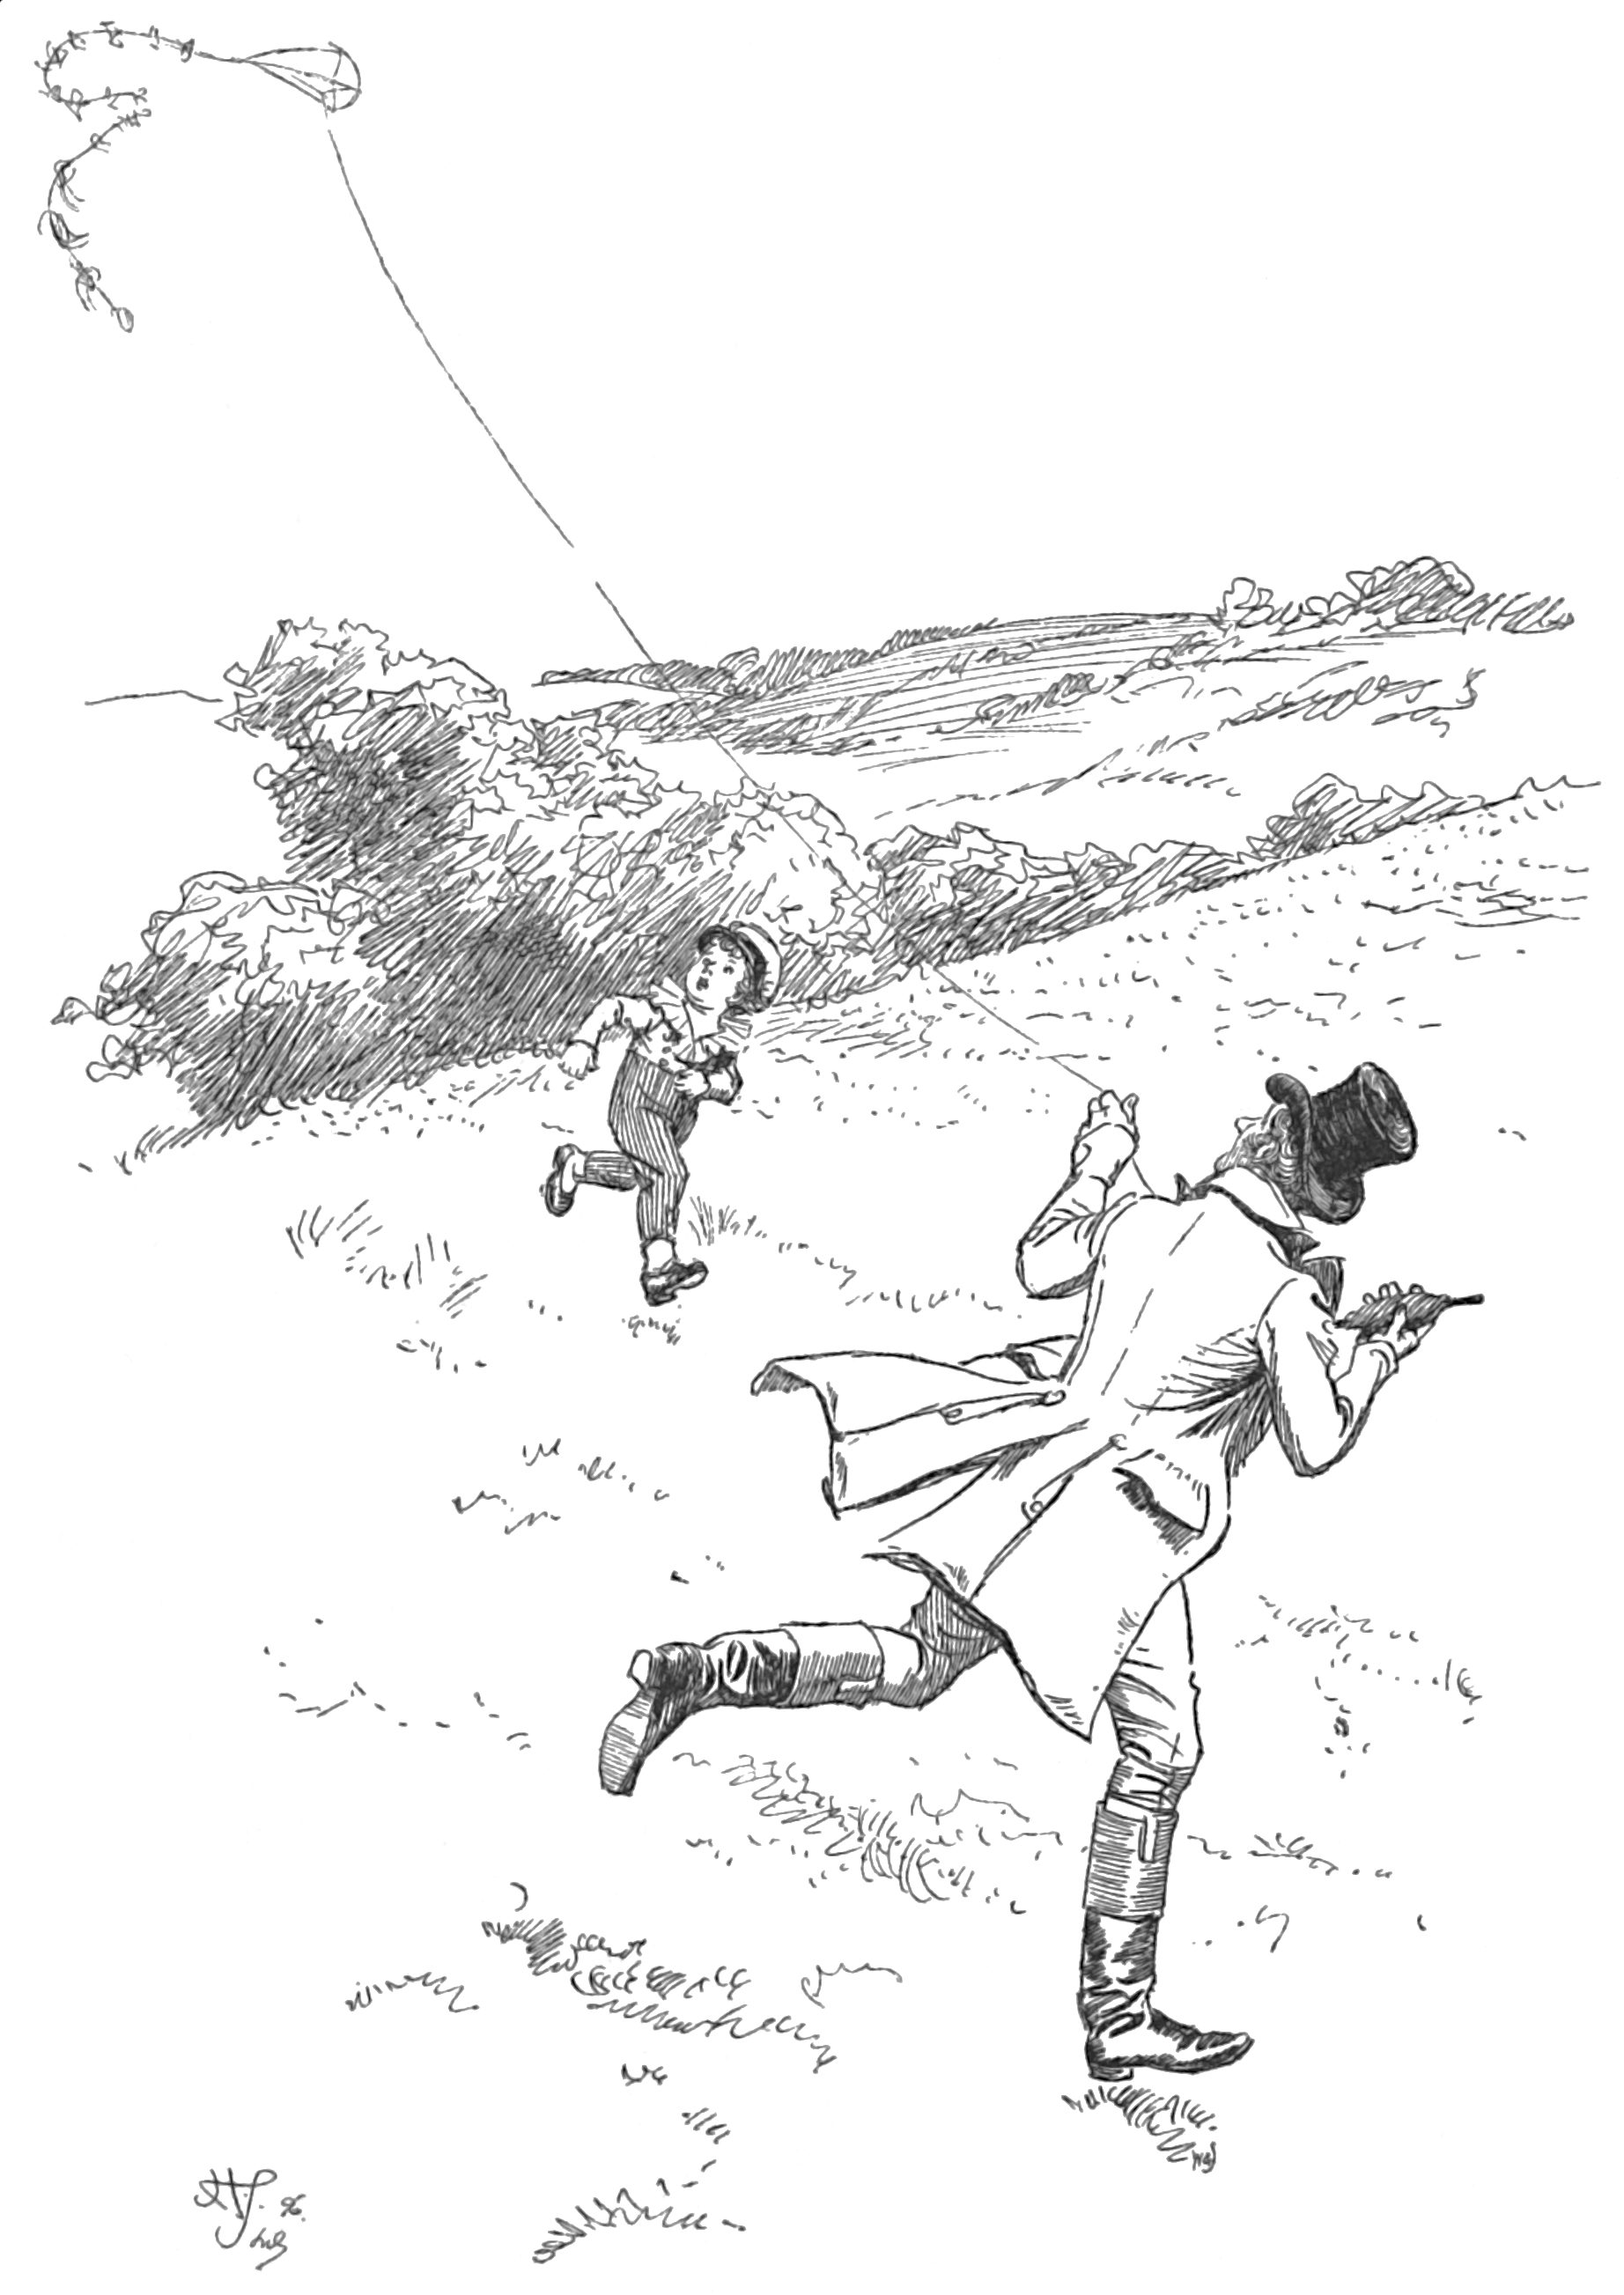
\includegraphics[width=.9\linewidth]{11kite}
\caption{Flying Henry's kite for him}
\end{figure}

<Me, my love,> cried his wife, hearing and understanding only in part.— <Are you talking about me?—I am sure nobody ought to be, or can be, a greater advocate for matrimony than I am; and if it had not been for the misery of her leaving Hartfield, I should never have thought of Miss Taylor but as the most fortunate woman in the world; and as to slighting Mr Weston, that excellent Mr Weston, I think there is nothing he does not deserve. I believe he is one of the very best-tempered men that ever existed. Excepting yourself and your brother, I do not know his equal for temper. I shall never forget his flying Henry's kite for him that very windy day last Easter—and ever since his particular kindness last September twelvemonth in writing that note, at twelve o'clock at night, on purpose to assure me that there was no scarlet fever at Cobham, I have been convinced there could not be a more feeling heart nor a better man in existence.—If any body can deserve him, it must be Miss Taylor.>

<Where is the young man?> said John Knightley. <Has he been here on this occasion—or has he not?>

<He has not been here yet,> replied Emma. <There was a strong expectation of his coming soon after the marriage, but it ended in nothing; and I have not heard him mentioned lately.>

<But you should tell them of the letter, my dear,> said her father. <He wrote a letter to poor Mrs Weston, to congratulate her, and a very proper, handsome letter it was. She shewed it to me. I thought it very well done of him indeed. Whether it was his own idea you know, one cannot tell. He is but young, and his uncle, perhaps\longdash>

<My dear papa, he is three-and-twenty. You forget how time passes.>

<Three-and-twenty!—is he indeed?—Well, I could not have thought it—and he was but two years old when he lost his poor mother! Well, time does fly indeed!—and my memory is very bad. However, it was an exceeding good, pretty letter, and gave Mr and Mrs Weston a great deal of pleasure. I remember it was written from Weymouth, and dated Sept. 28th—and began, <My dear Madam,> but I forget how it went on; and it was signed <F.~C. Weston Churchill.>—I remember that perfectly.>

<How very pleasing and proper of him!> cried the good-hearted Mrs John Knightley. <I have no doubt of his being a most amiable young man. But how sad it is that he should not live at home with his father! There is something so shocking in a child's being taken away from his parents and natural home! I never could comprehend how Mr Weston could part with him. To give up one's child! I really never could think well of any body who proposed such a thing to any body else.>

<Nobody ever did think well of the Churchills, I fancy,> observed Mr John Knightley coolly. <But you need not imagine Mr Weston to have felt what you would feel in giving up Henry or John. Mr Weston is rather an easy, cheerful-tempered man, than a man of strong feelings; he takes things as he finds them, and makes enjoyment of them somehow or other, depending, I suspect, much more upon what is called society for his comforts, that is, upon the power of eating and drinking, and playing whist with his neighbours five times a week, than upon family affection, or any thing that home affords.>

Emma could not like what bordered on a reflection on Mr Weston, and had half a mind to take it up; but she struggled, and let it pass. She would keep the peace if possible; and there was something honourable and valuable in the strong domestic habits, the all-sufficiency of home to himself, whence resulted her brother's disposition to look down on the common rate of social intercourse, and those to whom it was important.—It had a high claim to forbearance.